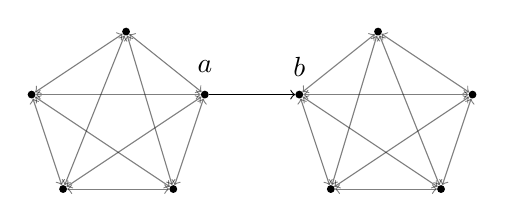
\begin{tikzpicture}[node distance=10pt]
\tikzstyle{blackdot} = [circle, fill, scale=0.3];
\tikzstyle{conn} = [<->,opacity=0.5];
\node [blackdot] (v1) at (-0.4,2) {};
\node [blackdot] (v2) at (-1.6,1.2) {};
\node [blackdot] (v3) at (-1.2,0) {};
\node [blackdot] (v4) at (0.2,0) {};
\node [blackdot] (v5) at (0.6,1.2) {};
\node [blackdot] (v6) at (1.8,1.2) {};
\node [blackdot] (v7) at (2.8,2) {};
\node [blackdot] (v8) at (4,1.2) {};
\node [blackdot] (v9) at (3.6,0) {};
\node [blackdot] (v10) at (2.2,0) {};
\draw [conn] (v1) edge (v2);
\draw [conn] (v2) edge (v3);
\draw [conn] (v3) edge (v4);
\draw [conn] (v5) edge (v4);
\draw [conn] (v5) edge (v1);
\draw [conn] (v2) edge (v5);
\draw [conn] (v5) edge (v3);
\draw [conn] (v3) edge (v1);
\draw [conn] (v4) edge (v1);
\draw [conn] (v4) edge (v2);
\draw [conn] (v6) edge (v7);
\draw [conn] (v7) edge (v8);
\draw [conn] (v9) edge (v8);
\draw [conn] (v10) edge (v9);
\draw [conn] (v10) edge (v6);
\draw [conn] (v6) edge (v8);
\draw [conn] (v8) edge (v10);
\draw [conn] (v10) edge (v7);
\draw [conn] (v7) edge (v9);
\draw [conn] (v9) edge (v6);
\draw [->] (v5) edge (v6);
\node [above of=v5] {$a$};
\node [above of=v6] {$b$};
\end{tikzpicture}